\documentclass[final]{beamer}
\mode<presentation> {  %% check http://www-i6.informatik.rwth-aachen.de/~dreuw/latexbeamerposter.php for examples
  \usetheme{I6pd}    %% you should define your own theme e.g. for big headlines using your own logos 
}
\usepackage[english]{babel}
\usepackage[latin1]{inputenc}
\usepackage{amsmath,amsthm, amssymb, latexsym}
\usepackage{array,booktabs,tabularx}
\usepackage{graphicx}
\usefonttheme[onlymath]{serif}
\boldmath
\usepackage[orientation=landscape,size=custom,width=200,height=120,scale=1.9,debug]{beamerposter}
\title{\huge Building Proteomic Application Platforms for Cloud Computing Environments with CloudBioLinux}
\author[Chilton, Zenka, et al]{Chilton, J.\textsuperscript{1}, Zenka, R.\textsuperscript{2}, Jagtap, P.\textsuperscript{1}, Lynch, B.\textsuperscript{1}, Bergen, H.R.\textsuperscript{2}, Griffin T.J.\textsuperscript{3}}
\institute[]{\textsuperscript{1}University of Minnesota Supcomputing Institute; \textsuperscript{2}Mayo Clinic; \textsuperscript{3}University of Minnesota}
\date{June 10th, 2013}

\newlength{\columnheight}
\setlength{\columnheight}{105cm}

\begin{document}
\begin{frame}
  \begin{columns}

    \begin{column}{.5\textwidth}
      \begin{beamercolorbox}[center,wd=\textwidth]{postercolumn}
        \begin{minipage}[T]{.95\textwidth}  % tweaks the width, makes a new \textwidth
          \parbox[t][\columnheight]{\textwidth}{
            \begin{block}{CloudBioLinux for Data Analysis}

            \begin{itemize}
            \item CloudBioLinux is an open-source framework for creating fully
            automated installation mechanisms for bioinformatics software and
            data.

            \item We have contributed numerous extensions and enhancements to
            CloudBioLinux to make a great environment for building mass spec data analysis
            platforms.

            \item With emerging proteomics applications such as
            proteogenomics, it is becoming essential to build applications
            platforms that tie together traditional proteomic analyses
            with other bioinformatic analyses (such as sequence similarity 
            analysis or genomic mapping). CloudBioLinux is an ideal platform 
            for creating such platforms.

            \end{itemize}

            \end{block}

            \vfill
            \begin{block}{https://biocloudcentral.msi.umn.edu/ - Create Your Own Cluster}
              \begin{columns}
                \begin{column}{.35\textwidth}
                  \begin{figure}
                    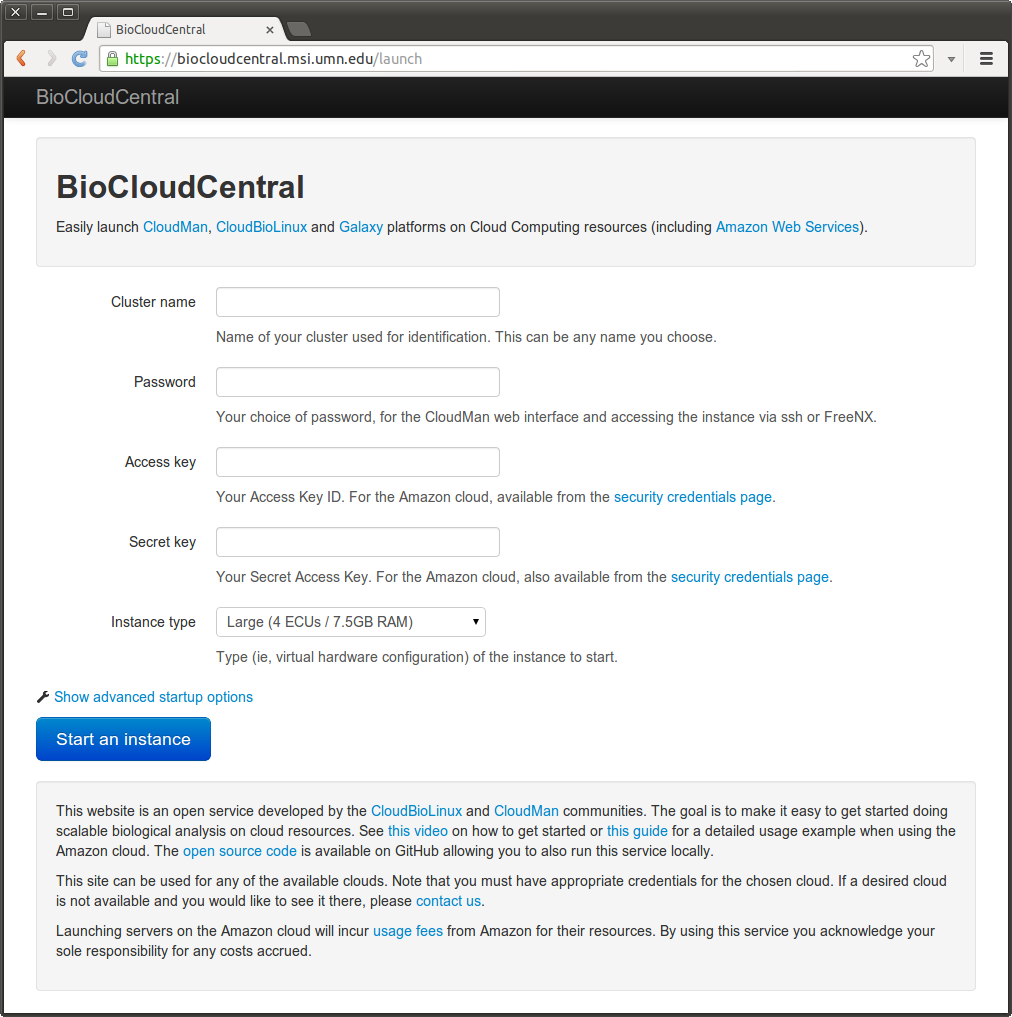
\includegraphics[scale=0.5]{biocloudcentral.png}
                  \end{figure}              
                \end{column}

                \begin{column}{.60\textwidth}
                  \begin{itemize}

                    \item Spin up your own cluster created with CloudBioLinux
                    and customized for mass spec data analysis today at
                    https://biocloudcentral.msi.umn.edu.

                    \item All you need is your Amazon Web Services (AWS)
                    credentials and BioCloudCentral will orchestrate the creation
                    of a cluster on Amazon EC2 for your data analysis.

                    \item Cluster is preconfigured with CloudMan an easy-to-
                    use interface for managing your new Amazon cluster.

                  \end{itemize}
                \end{column}

              \end{columns}

            \end{block}

            \vfill

            \begin{columns}
              \begin{column}{.49\textwidth}
            
            \begin{block}{Applications}
              \begin{description}
                 \item[\textbf{Large Proteomic Tool Suites}] \hfill \\
                  \textsl{Trans proteomic-pipeline, OpenMS, crux}
                \item[\textbf{Datbase Search Tools}] \hfill \\
                  \textsl{Myrimatch, X! Tandem, OMSSA, ...}
                \item[\textbf{Specialized Identification Tools}] \hfill \\
                  \textsl{TagRecon, PepNovo, ...}
                \item[\textbf{Validation Tools}] \hfill \\
                  \textsl{Percolator, Fido, Mayu, ...}
                \item[\textbf{Bioinformatics}] \hfill \\
                  \textsl{NCBI Blast+, EMBOSS, Augustus, ...}
                \item[\textbf{Tools Developed at the University of Minnesota}]  \hfill \\
                  \textsl{iQuant (isobaric quantification), psm-eval (flexiable re-evaluation of identified peptide-spectrum matches), peptide-to-gff (map peptides for genomic visualization)}
              \end{description}
            \end{block}
              \end{column}
              \begin{column}{.02\textwidth}
              \end{column}
              \begin{column}{.49\textwidth}
            \begin{block}{Programming Libraries}

              \begin{description}
                 \item[\textbf{pyteomics}] \hfill \\
                  \textsl{"Pyteomics provides a growing set of modules to facilitate the most common tasks in proteomics data analysis..." }\\
                  https://pypi.python.org/pypi/pyteomics
                \item[\textbf{mspire}] \hfill \\
                  \textsl{"Mspire is a full featured library for working with mass spectrometry data, particularly proteomic, metabolomic and lipidomic data sets."} \\
                  https://github.com/princelab/mspire
                \item[\textbf{R}] \hfill \\
                  Our preconfigured CloudBioLinux image comes preinstalled with various useful R libraries proteomic data analysis
                  ({\textsl e.g. xcms, mzR, FactoMineR, caret, ggplot2, VennDiagram, ...})
              \end{description}
            \end{block}

              \end{column}
            \end{columns}
            \vfill
            \begin{block}{Graphical Applications}

            \begin{columns}
              \begin{column}{.30\textwidth}
                \begin{figure}
                  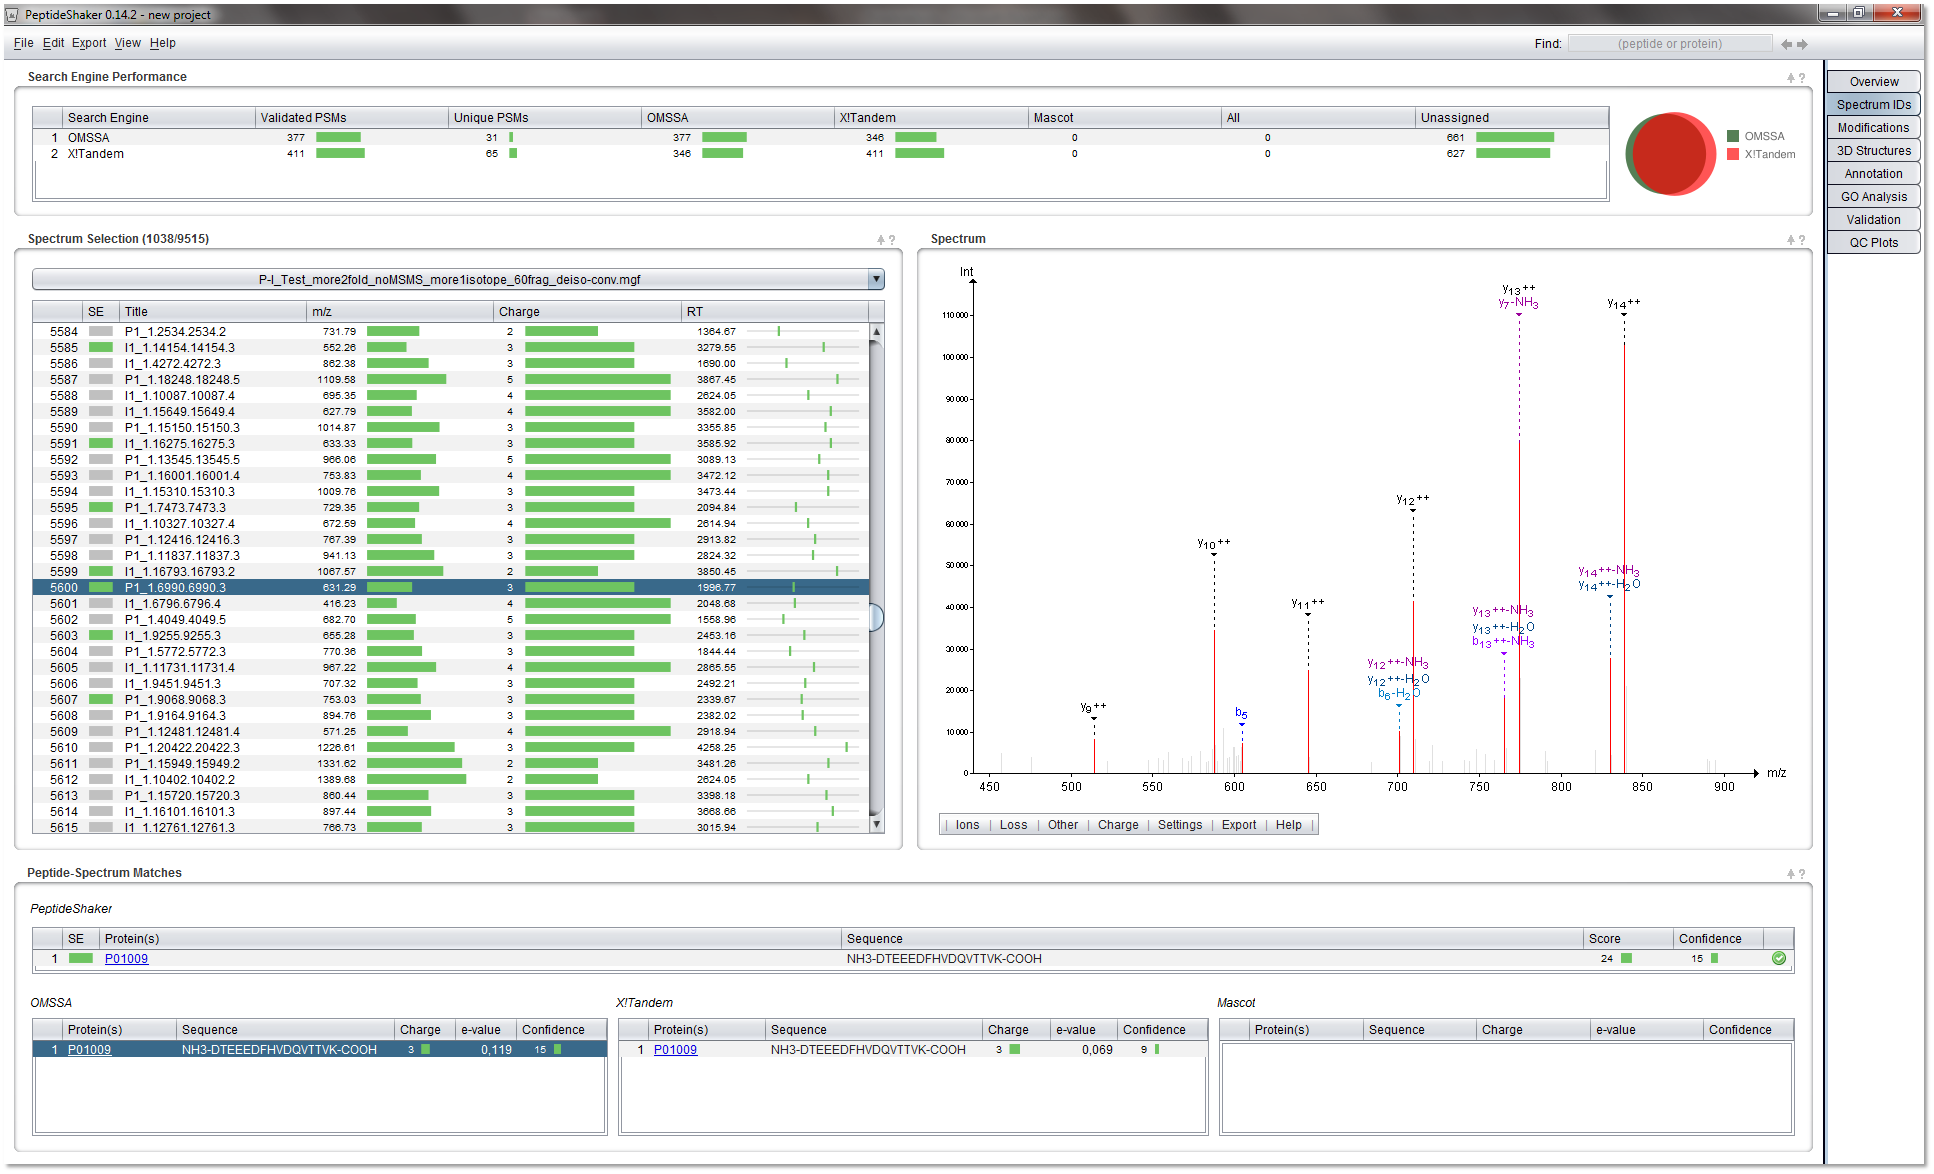
\includegraphics[scale=0.4]{peptideshaker_screenshot_fake.png} \\
                  \caption{TODO: Replace me with actual screenshot from a Cloud environment.}
                \end{figure}                   
              \end{column}
              \begin{column}{.39\textwidth}
                Our example CloudBioLinux environment comes bundled with user-friendly graphical Desktop applications as well.
                \begin{itemize}
                  \item MZmine
                  \item PeptideShaker and SearchGUI
                  \item TOPPAS
                  \item PRIDE Converter
                  \item PRIDEInspector
                \end{itemize}
              \end{column}
              \begin{column}{.30\textwidth}
                \begin{figure}
                  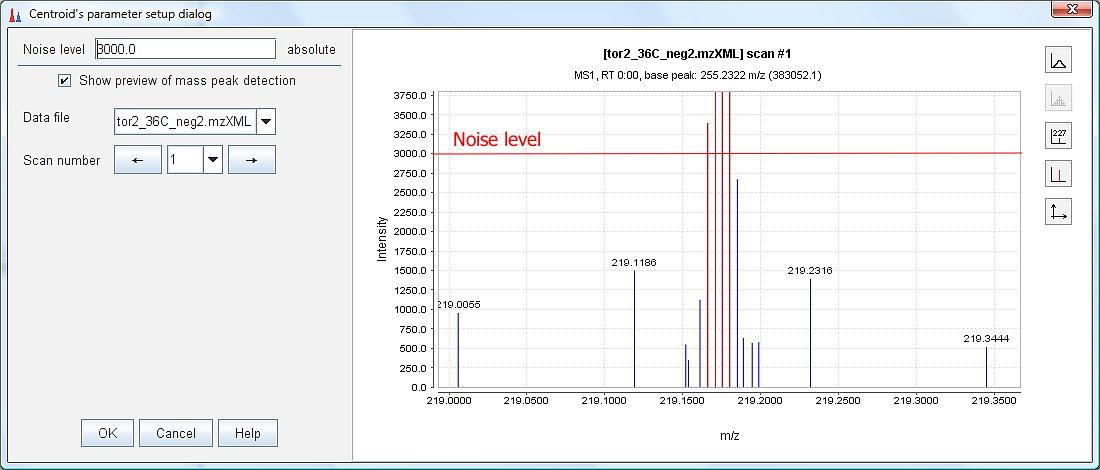
\includegraphics[scale=0.5]{mzmine_screenshot_fake.jpg}
                  \caption{TODO: Replace me with actual screenshot from a Cloud environment.}
                \end{figure}
              \end{column}              
            \end{columns}
            \end{block}
          }
        \end{minipage}
      \end{beamercolorbox}
    \end{column}

    \begin{column}{.5\textwidth}
      \begin{beamercolorbox}[center,wd=\textwidth]{postercolumn}
        \begin{minipage}[T]{.95\textwidth} % tweaks the width, makes a new \textwidth
          \parbox[t][\columnheight]{\textwidth}{
            \begin{block}{CloudBioLinux for Platform Development}

            Check out you own copy of CloudBioLinux on Github at
            https://github.com/chapmanb/cloudbiolinux and build a customized
            flavor for your mass spec data analysis platform.

            \begin{itemize}
            \item Simple YAML data files describe what software, libraries, 
            and data to install.

            \item Integrate your own applications (big or small) using native OS
            packages, fabric functions, Puppet modules, or Chef cookbooks.
            \end{itemize}

            \end{block}

            \vfill
            
            \begin{block}{CloudBioLinux as a Platform - wine}

              \begin{columns}
                \begin{column}{.40\textwidth}
                  \begin{figure}
                    \includegraphics[scale=.9]{morpheus_screenshot.png} 
                    \caption{Screenshot of the Windows-only software Morpheus running under Linux using Wine}
                  \end{figure}
                \end{column}
                \begin{column}{.59\textwidth}
                  \begin{itemize}

            \item Wine is a compatibility layer allowing many Windows applications
            to run other other operating systems (such as Linux). 
            
            \item We have built a high level framework for packaging and
            redistributing Wine enviornments. https://github.com/jmchilton/proteomics-wine-env \hfill \\


            \hskip2cm Includes documentation for creating such a Wine environment
            and configuring msconvert to work with vendor libraries.

            \item CloudBioLinux includes support for distributing such
            environments and creating friendly wrapper scripts along with install
            procedures for proteomics programs such as msconvert and multiplierz.

            \end{itemize}
            \end{column}
            \end{columns}
            \end{block}

            \vfill
            
            \begin{block}{CloudBioLinux as a Platform - Galaxy-P}

              \begin{columns}

                \begin{column}{.60\textwidth}
                  \begin{itemize}

                    \item  Galaxy-P (http://getgalaxyp.org) is an extension to the popular Galaxy framework to 
                    enable proteomics workflows.

                    \item The example image that can be launched with CloudBioLinux comes preconfigured with 
                    an a subset of Galaxy-P.


                    \item The cross-disciplinary nature of Galaxy-P demonstrates the utility of building on 
                    CloudBioLinux and the complexity of Galaxy-P demonstrates the necessity for automating such 
                    deployments.

                    \item Our internal and public Galaxy server (https://usegalaxyp.org)

                  \end{itemize}
                \end{column}

                \begin{column}{.35\textwidth}
                  \begin{figure}
                    \includegraphics[scale=0.7]{galaxyp_screenshot.png}
                  \end{figure}
                \end{column}

              \end{columns}

            \end{block}


            \vfill
            
            \begin{block}{CloudBioLinux as a Platform - Swift}
            \vfill

            \VeryHuge{Roman's \\ ......SWIFT  \\ ...........content.}

            \vfill

            \end{block}
          }
        \end{minipage}
      \end{beamercolorbox}
    \end{column}              

  \end{columns}   
\end{frame}
\end{document}
